\ifx\allfiles\undefined
\documentclass[12pt, a4paper, oneside, UTF8]{ctexbook}  % +  这一句是新增加的
\usepackage{amsmath}   % 数学公式
\usepackage[dvipsnames]{xcolor}
\usepackage{amsthm}    % 定理环境
\usepackage{amssymb}   % 更多公式符号
\usepackage{graphicx}  % 插图
\usepackage{mathrsfs}  % 数学字体
\usepackage{enumitem}  % 列表
\usepackage{geometry}  % 页面调整
\usepackage{unicode-math}
\usepackage{extarrows}
\usepackage{subfigure}
\usepackage{extarrows}
\usepackage{footnote}
\usepackage{svg}
\usepackage[colorlinks,linkcolor=black]{hyperref}
\usepackage{supertabular}
\usepackage{tcolorbox}
\usepackage{ulem}
\usepackage{framed}
\usepackage{float}
\usepackage{microtype}
\newcommand{\arccot}{\mathrm{arccot}\,}
\tcbuselibrary{breakable}
\tcbuselibrary{most}
\newcounter{problemname}
\newenvironment{solution}{\par\noindent\textbf{解答. }}{\par}
\newenvironment{note}{\par\noindent\textbf{题目\arabic{problemname}的注记. }}{\par}
\definecolor{shadecolor}{RGB}{241, 241, 255}
\newenvironment{problem}{\begin{shaded}\stepcounter{problemname}\par\noindent\textbf{题目\arabic{problemname}. }}{\end{shaded}\par}

\graphicspath{ {figure/},{../figure/}, {config/}, {../config/} }  % 配置图形文件检索目录
\linespread{1.2} % 行高

% 页码设置
\geometry{top=25.4mm,bottom=25.4mm,left=20mm,right=20mm,headheight=2.17cm,headsep=4mm,footskip=12mm}

% 设置列表环境的上下间距
\setenumerate[1]{itemsep=5pt,partopsep=0pt,parsep=\parskip,topsep=5pt}
\setitemize[1]{itemsep=5pt,partopsep=0pt,parsep=\parskip,topsep=5pt}
\setdescription{itemsep=5pt,partopsep=0pt,parsep=\parskip,topsep=5pt}

% 定理环境
% ########## 定理环境 start ####################################

% #### 将 config.tex 中的定理环境的对应部分替换为如下内容
% 定义单独编号,其他四个共用一个编号计数 这里只列举了五种,其他可类似定义(未定义的使用原来的也可)
\newtcbtheorem[auto counter, number within=section, list type=subsubsection, list inside=toc]{defn}{定义}
{
    colback=green!5,colframe=green!35!black,fonttitle=\bfseries, title={Comment \thetcbcounter}, list entry={Comment \thetcbcounter\quad}, %标题
    breakable, %支持跨页
    before upper={\parindent10pt\noindent},  % 支持缩进。\noindent:首行不缩进
    % left = 2mm, %文字离线框左边的边距
    % right = 1mm,%同上
    % top = 1mm,%同上
    % bottom = 1mm,%同上
    % arc is angular = 1mm, % 棱角线框
    % sharp corners, % 直角线框
    % enhanced,frame hidden, % 隐藏线框
    % enhanced, drop fuzzy shadow,  % 显示阴影
}
{def}

\newtcbtheorem[auto counter, number within=section, list type=subsubsection, list inside=toc]{lemma}{引理}
{
    colback=SeaGreen!10!CornflowerBlue!10,colframe=RoyalPurple!55!Aquamarine!100!,fonttitle=\bfseries, title={Comment \thetcbcounter}, list entry={Comment \thetcbcounter\quad}, %标题
    breakable, %支持跨页
    before upper={\parindent10pt\noindent},  % 支持缩进。\noindent:首行不缩进
    % left = 2mm, %文字离线框左边的边距
    % right = 1mm,%同上
    % top = 1mm,%同上
    % bottom = 1mm,%同上
    % arc is angular = 1mm, % 棱角线框
    % sharp corners, % 直角线框
    % enhanced,frame hidden, % 隐藏线框
    % enhanced, drop fuzzy shadow,  % 显示阴影
}
{lem}


\newtcbtheorem[auto counter, number within=section, list type=subsubsection, list inside=toc]{them}{定理}
{
    colback=Salmon!20, colframe=Salmon!90!Black,fonttitle=\bfseries, title={Comment \thetcbcounter}, list entry={Comment \thetcbcounter\quad}, %标题
    breakable, %支持跨页
    before upper={\parindent10pt\noindent},  % 支持缩进。\noindent:首行不缩进
    % left = 2mm, %文字离线框左边的边距
    % right = 1mm,%同上
    % top = 1mm,%同上
    % bottom = 1mm,%同上
    % arc is angular = 1mm, % 棱角线框
    % sharp corners, % 直角线框
    % enhanced,frame hidden, % 隐藏线框
    % enhanced, drop fuzzy shadow,  % 显示阴影
}
{them}
\newtcbtheorem[auto counter, number within=section, list type=subsubsection, list inside=toc]{criterion}{注}
{
    colback=CornflowerBlue!10,colframe=RoyalPurple!55!Aquamarine!100!,fonttitle=\bfseries, title={Comment \thetcbcounter}, list entry={Comment \thetcbcounter\quad}, %标题
    breakable, %支持跨页
    before upper={\parindent10pt\noindent},  % 支持缩进。\noindent:首行不缩进
    % left = 2mm, %文字离线框左边的边距
    % right = 1mm,%同上
    % top = 1mm,%同上
    % bottom = 1mm,%同上
    % arc is angular = 1mm, % 棱角线框
    % sharp corners, % 直角线框
    % enhanced,frame hidden, % 隐藏线框
    % enhanced, drop fuzzy shadow,  % 显示阴影
}
{cri}

\newtcbtheorem[auto counter, number within=section, list type=subsubsection, list inside=toc]{corollary}{推论}
{
    colback=Emerald!10,colframe=cyan!40!black,fonttitle=\bfseries, title={Comment \thetcbcounter}, list entry={Comment \thetcbcounter\quad}, %标题
    breakable, %支持跨页
    before upper={\parindent10pt\noindent},  % 支持缩进。\noindent:首行不缩进
    % left = 2mm, %文字离线框左边的边距
    % right = 1mm,%同上
    % top = 1mm,%同上
    % bottom = 1mm,%同上
    % arc is angular = 1mm, % 棱角线框
    % sharp corners, % 直角线框
    % enhanced,frame hidden, % 隐藏线框
    % enhanced, drop fuzzy shadow,  % 显示阴影
}
{cor}
% colback=red!5,colframe=red!75!black

% ######### 定理环境 end  #####################################

% ↓↓↓↓↓↓↓↓↓↓↓↓↓↓↓↓↓ 以下是自定义的命令  ↓↓↓↓↓↓↓↓↓↓↓↓↓↓↓↓

% 用于调整表格的高度  使用 \hline\xrowht{25pt}
\newcommand{\xrowht}[2][0]{\addstackgap[.5\dimexpr#2\relax]{\vphantom{#1}}}

% 表格环境内长内容换行  
\newcommand{\tabincell}[2]{\begin{tabular}{@{}#1@{}}#2\end{tabular}}

% 使用\linespread{1.5} 之后 cases 环境的行高也会改变,重新定义一个 ca 环境可以自动控制 cases 环境行高
\newenvironment{ca}[1][1]{\linespread{#1} \selectfont \begin{cases}}{\end{cases}}
% 和上面一样
\newenvironment{vx}[1][1]{\linespread{#1} \selectfont \begin{vmatrix}}{\end{vmatrix}}

\def\d{\textup{d}} % 直立体 d 用于微分符号 dx
\def\R{\mathbb{R}} % 实数域
\newcommand{\bs}[1]{\boldsymbol{#1}}    % 加粗,常用于向量
\newcommand{\ora}[1]{\overrightarrow{#1}} % 向量

% 数学 平行 符号
\newcommand{\pll}{\kern 0.5em/\kern -0.8em /\kern 0.5em}

% 用于空行\myspace{1} 表示空一行 填 2 表示空两行  
\newcommand{\myspace}[1]{\par\vspace{#1\baselineskip}}

\begin{document}
\begin{sloppypar}
    % \title{{\Huge{\textbf{高等数学笔记}}}}
\author{作者:于家崇}
\date{\today}
\maketitle                   % 在单独的标题页上生成一个标题

\thispagestyle{empty}        % 前言页面不使用页码
\begin{center}
	\Huge\textbf{前言}
\end{center}

If a job is worth doing,it's worth doing well
\begin{flushright}
	\begin{tabular}{c}
		\today \\ 如果一件事值得去做,那就值得去做好
	\end{tabular}
\end{flushright}

\newpage                      % 新的一页
\pagestyle{plain}             % 设置页眉和页脚的排版方式(plain:页眉是空的,页脚只包含一个居中的页码)
\setcounter{page}{1}          % 重新定义页码从第一页开始
\pagenumbering{Roman}         % 使用大写的罗马数字作为页码
\tableofcontents              % 生成目录

\newpage                      % 以下是正文
\pagestyle{plain}
\setcounter{page}{1}          % 使用阿拉伯数字作为页码
\pagenumbering{arabic}
% \setcounter{chapter}{-1}    % 设置 -1 可作为第零章绪论从第零章开始 
    \else
    \fi
    %  ############################ 正文部分
    \chapter{极限}
    \section{数列的极限}
    \subsection{数列极限的定义}
    \begin{defn}{}{}
        设$|x_n|$为一数列,若\uwave{存在常数$a$},对于\uwave{任意的$\varepsilon>0$(不论它多么小)},\uwave{总存在正整数$N$},使得当\uwave{$n>N$}时 \uwave{$|x_n-a|<\varepsilon$ 恒成立},则称数 $a$是数列$| x_n |$的极限,或者称数列$| x_n |$收敛于 $a$,记为
        $$
            \lim_{n\to\infty}x_n=a\text{ 或 }x_n\to a(n\to\infty).
        $$
        该定义的$\varepsilon-N$语言描述是\\
        $$\lim_{n\to\infty}x_n=a\Leftrightarrow\forall\varepsilon>0,\exists\text{正整数}N,\text{当}n>N\text{时},\text{有}|x_n,-a|<\varepsilon.$$
        其中$\forall\varepsilon>0$是白给的信息,随便写.$\exists\text{正整数}N$是关键.因为第二句话说的是一定存在正整数N,你怎么才能够证明存在正整数N呢?那就必须把这个正整数N给找出来,你找出来才能够证明这个N是存在的.关键第三句话叫做桥梁,桥梁什么意思?就是n大于N的时候n大于N的时候,也就意味着N趋近于无穷的过程中.在大N项之后的所有的项.最后一句话叫做突破口.,不是要去找这个N吗?你找到N才能够证明这个N是存在的,我们一般情况下就用第四句话来寻找大N.
    \end{defn}
    在上面的定义中,$\varepsilon>0$的$\varepsilon$任意性是非常重要的,只有这样才能表示出\textcolor{red}{无限接近的意义}.总存在正整数$N$,使得$n>N$这个条件用于表达$n \to \infty$的过程.
    \begin{criterion}{}{}
        \begin{itemize}
            \item 数列的极限值与数列的前有限列无关,只与后面无穷项有关
            \item $\underset{n\to\infty}{\operatorname*{\lim}}x_n=a\Leftrightarrow\underset{k\to\infty}{\operatorname*{\lim}}x_{2k-1}=\underset{k\to\infty}{\operatorname*{\lim}}x_{2k}=a$
            \item $\varepsilon - N$\textbf{几何意义: 对于点$a$的任何$\varepsilon$邻域即开区间$(a-\varepsilon,a+\varepsilon)$一定存在$N$,当$n < N$即第$N$项以后的点$x_n$都落在开区间$(a-\varepsilon,a+\varepsilon)$内,而只有有限个(最多有$N$个)在区间之外.}
        \end{itemize}
    \end{criterion}

    \begin{problem}
    已知$x_{n}=\frac{\left(\begin{array}{c}-1\\\end{array}\right)^{n}}{\left(\begin{array}{c}n+1\\\end{array}\right)^{2}}$,证明数列${x_n}$的极限是$0$
    \end{problem}
    \begin{note}
        根据数列极限的定义可知,$\forall\varepsilon>0,\exists\text{正整数 }N,\text{当 }n{>}N\text{ 时 },\text{有}|x_{n} - 0 =\frac{\left(\begin{array}{c}-1\\\end{array}\right)^{n}}{\left(\begin{array}{c}n+1\\\end{array}\right)^{2}}|<\varepsilon.$,即$x_{n}=\frac{\begin{array}{c}1\\\end{array}}{\left(\begin{array}{c}n+1\\\end{array}\right)^{2}} < \varepsilon \Leftrightarrow \frac{1}{n^2}< \varepsilon \Leftrightarrow n > \frac{1}{\sqrt{\varepsilon}}$,即令$N > \frac{1}{\sqrt{\varepsilon}}$,$\frac{1}{\sqrt{\varepsilon}}$是一个确定的实数,大于它的正整数有无穷个,仍取其中一个作为$N$即可.
    \end{note}
    \begin{solution}
        $\forall \varepsilon>0$,取$N=\frac{1}{\sqrt{\varepsilon}}+1$,则总有$x_{n}=\frac{\begin{array}{c}1\\\end{array}}{\left(\begin{array}{c}n+1\\\end{array}\right)^{2}} < \varepsilon \Leftrightarrow \frac{1}{n^2}< \varepsilon \Leftrightarrow n > \frac{1}{\sqrt{\varepsilon}}$,则数列${x_n}$的极限是$0$
    \end{solution}
    \subsection{收敛数列的性质}
    \subsubsection{唯一性}
    \begin{them}{}{}
        如果数列$\{ x_n \}$收敛,那么它的极限唯一
    \end{them}
    \subsubsection{有界性}
    \begin{them}{}{}
        如果数列$\{x_n\}$收敛,那么数列$\{x_n\}$一定有界.
    \end{them}
    \begin{criterion}{}{}
        需要注意的是,如果数列有界,但是不一定存在极限,如数列$(-1)^n$
    \end{criterion}
    \subsubsection{保号性}
    \begin{them}{}{}
        $\text{如果}\lim_{n\to\infty}x_n=a,\text{且}a{>}0(\text{ 或 }a{<}0),\text{那么存在正整数 }N,\text{当 }n{>}N\text{ 时 },\text{都有 }x_n{>}0\left(\text{ 或 }x_n{<}0\right)$
    \end{them}
    \begin{corollary}{}{}
        $\text{如果数列}\mid x_n\mid\text{从某项起有 }x_n\geqslant0\text{(或 }x_n\leqslant0\text{)},\text{且}\lim_{n\to\infty}x_n=a\text{ ,那么 }a\geqslant0(\text{ 或 }a\leqslant0).$
    \end{corollary}
    \subsubsection{收敛数列与其子数列之间的关系}
    如果数列${x_n}$收敛于$a$,那么它的任一子数列也收敛,且极限也是$a$
    \begin{criterion}{}{}
        需要注意的是,证明数列极限存在一般通过证明数列有界并且单调,证明有界则一般通过放缩法.但是证明数列发散则一般通过一下两种方法:1.至少一个子数列发散.2.两个子数列收敛,但是收敛值不同.
    \end{criterion}
    \section{函数的极限}
    \subsection{超实数系}
    \begin{defn}{超实数系的概念}{}
        超实数(Hyperreal number)是一个包含实数以及无穷大和无穷小的域,它们的绝对值分别大于和小于任何正实数。
    \end{defn}
    \begin{criterion}{}{}
        \begin{itemize}
            \item 超实数集\textbf{是为了严格处理无穷量(无穷大量和无穷小量)而提出的}。
            \item 超实数集,或称为非标准实数集,记为$^{*}\mathbb{R}$,是实数集$\mathbb{R}$的一个扩张.
        \end{itemize}
    \end{criterion}
    \subsection{邻域}\footnote{邻域与区间不同,邻域属于区间的范畴.但是邻域通常表示“一个局部位置”.比如“点$x_0$的$\delta$”邻域,可以理解为“点$x_0$”的附近,而区间是明确指出在实数系下的范围}
    \begin{defn}{邻域的相关概念}{}
        \begin{itemize}
            \item $\delta$邻域:设$x_0$是数轴上一个点,$\delta$是某一正数,则称$(x_{0}-\delta,x_{0}+\delta)$为点$x_0$的$\delta$邻域,记作$U(x_{0},\delta)$,即:
                  $$
                      U(x_{0},\delta)=\left\{x|x_{0}-\delta<x<x_{0}+\delta\right\}=\left\{\left.x\right|\left|\left.x-x_{0}\right|<\delta\right\}\right.
                  $$
            \item 去心$\delta$邻域:定义点$x_0$的去心邻域$\mathring{U}(x_{0},\delta)=\bigl\{x|0<\bigl|x-x_{0}\bigr|<\delta\bigr\}$
            \item 左,右$\delta$邻域:$\left\{x|0<x-x_{0}<\delta\right\}$称为点$x_0$的右$\delta$邻域,记作$U^{+}(x_{0},\delta);\{x|0<x_{0}-x<\delta\}$称为点$x_0$的左$\delta$邻域,记作$U^{-}(x_{0},\delta).$
        \end{itemize}
    \end{defn}
    \subsection{函数极限的定义}
    函数极限的定义主要分为自变量趋于有限值$(x \to x_0)$时的极限和自变量趋于无穷大时函数的极限$(x \to \infty)$
    \subsubsection{自变量趋于有限值时的函数极限}
    \begin{defn}{当自变量趋于有限值时函数极限定义}{}
        设函数$f(x)$在点$x_0$的某一去心邻域内有定义.如果存在常数$A$,对于任意给定的正数$\varepsilon$\textbf{(不论它多么小)\footnote{$\varepsilon$用于衡量$|f(x)-A|$的值有多小}},总存在正数$\delta$,使得当$x$满足不等式$0<|x-x_0|<\delta$时,对应的函数值$f(x)$都满足不等式
        $$
            |f(x)-A|<\varepsilon
        $$
        那么常数$A$就叫做\uwave{函数$f(x)$当$x \to x_0$时的极限},记作:
        $$
            \lim_{x\to x_0}f(x)=A\quad\text{或}f(x)\to A(\text{当}x\to x_0)
        $$
        其$\varepsilon-N$语言为
        $$
            \lim_{x\to x_0}f(x)=A\Leftrightarrow\forall\varepsilon>0,\exists\delta>0,\text{当}0<|x-x_0|<\delta\text{时},\text{有}|f(x)-A|<\varepsilon.
        $$
        $\forall\varepsilon>0,\exists\delta>0$在证明中,这两句是白给,直接写。后面的才是关键。
    \end{defn}
    \begin{criterion}{}{}
        在函数极限中$x \to \infty$指的是$|x| \to \infty$,需要$x$趋于正无穷和负无穷,但在数列中的$n \to \infty$是$n \to +\infty$
    \end{criterion}

    \subsubsection{单侧极限}
    \begin{defn}{单侧极限的定义}{}
        若当$x\to x_0^{-}$时,$f(x)$无限接近于某常数$A$,则常数$A$叫作函数$f(x)$当$x\to x_0$时的\textbf{左极限},记为
        \begin{center}
            $\operatorname*{lim}_{x\to x_0^{-}}f(x)=A$或 $f(x_0^{-})=A$.
        \end{center}
        若当$x\to x_0^+$时,$f(x)$无限接近于某常数$A$,则常数$A$叫作函数$f(x)$当$x\to x_0$时的\textbf{右极限},记为
        \begin{center}
            $\operatorname*{lim}_{x\to x_0^{+}}f(x)=A$或 $f(x_0^{+})=A$
        \end{center}
    \end{defn}
    \begin{problem}
    $\text{已知}\lim_{x\to0}\biggl[a\arctan\frac{1}{x}+(1+\mid x\mid)^{\frac{1}{x}}\biggr]\text{存在,求}a\text{的值}$
    \end{problem}
    \begin{solution}
        由于存在$\arctan$与$|x|$函数,则对于0点的极限值需要分左右进行计算.

        $\lim\limits_{x\to0^{-}}\left[\begin{matrix}a\arctan\frac{1}{x}+(1+\mid x\mid)^{\frac{1}{x}}\\\end{matrix}\right]=\lim\limits_{x\to0^{-}}a\arctan\frac{1}{x}+\lim\limits_{x\to0^{-}}(1-x)^{\frac{1}{x}}=-\frac{\pi}{2}a+\frac{1}{\text{e}}$

        $\lim\limits_{x\to0^+}\left[\begin{matrix}a\arctan\frac{1}{x}+(1+\mid x\mid)^{\frac{1}{x}}\\\end{matrix}\right]=\lim\limits_{x\to0^+}a\arctan\frac{1}{x}+\lim\limits_{x\to0^+}(1+x)^{\frac{1}{x}}=\frac{\pi}{2}a+\mathrm{e}$
        若极限存在,则$a=\frac{1-e^2}{\pi e}$
    \end{solution}
    \subsubsection{自变量趋于无穷大时函数的极限}
    \begin{defn}{自变量趋于无穷大时函数极限定义}{}
        设函数$f(x)$在点$x_0$的某一去心邻域内有定义.如果存在常数$A$,对于任意给定的正数$\varepsilon$.(不论它多么小),总存在正数$\delta$,使得当$x$满足不等式$0<|x-x_0|<\delta$时,对应的函数值$f(x)$都满足不等式
        $$
            |f(x)-A|<\varepsilon
        $$
        那么常数$A$叫做函数$f(x)$当$x \to x_0$的极限,记作:
        $$
            \lim_{x\to x_0}f(x)=A\text{或}f(x)\to A(\text{当}x\to x_0)
        $$
        其$\varepsilon-N$语言为
        $$
            \lim\limits_{x\to x_0}f(x)=A\Leftrightarrow\forall\varepsilon>0,\exists\delta>0,\text{当}0<|x-x_0|<\delta\text{时},\text{有}|f(x)-A|<\varepsilon.
        $$
        $\forall\varepsilon>0,\exists\delta>0$在证明中,这两句是白给,直接写。后面的才是关键。
    \end{defn}
    \textcolor{red}{需要注意的是趋向的值不同时,$\varepsilon -N$写法不同,不能照抄}.其$\varepsilon -N$的表达为如下表格:
    \begin{center}
        \tablefirsthead{
            \hline
            \textbf{} & \textbf{$f(x)\to A$} & \textbf{$f(x)\to \infty$} & \textbf{$f(x)\to +\infty$} & \textbf{$f(x)\to -\infty$}\\
            \hline
        }
        \tablehead{
            \hline
            \textbf{} & \textbf{$f(x)\to A$} & \textbf{$f(x)\to \infty$} & \textbf{$f(x)\to +\infty$} & \textbf{$f(x)\to -\infty$}\\
            \hline
        }
        \tabletail{
            \hline
        }
        \tablelasttail{
            \multicolumn{1}{r}{{继续下一页}} \\
        }
        \begin{supertabular}{|c|c|c|c|c|}
            \hline
            $x \to x_0$       & $\begin{aligned}&\forall\varepsilon>0,\exists\delta>0, \\&\text{使当 }0<\mid x-x_0\mid  \\&<\delta\text{ 时 },\text{即有} \\&|f(x)-A|<\varepsilon.\end{aligned}$ & $\begin{aligned}&\forall M>0,\exists\delta>0, \\&\text{使当 }0<\mid x-x_{0}\mid  \\&<\delta\text{ 时 },\text{即有}\\& |f(x)|>M\end{aligned}$ & $\begin{aligned}&\forall M>0,\exists\delta>0, \\&\text{使当} 0<|x-x_0| \\ &<\delta \text{时 ,即有} \\ &f(x)>M.\end{aligned}$      & $\begin{aligned}&\forall M>0,\exists\delta>0, \\&\text{使当 }0<\mid x-x_{0}\mid  \\&<\delta\text{ 时 ,即有}\\& f(x) <-M\end{aligned}$ \\ \hline
            $x \to x_0^+$     & $\begin{aligned}&\forall\varepsilon>0,\exists\delta>0, \\&\text{使当 }0<x-x_{0}< \\&\delta \text{时,即有}\\&|f(x)-A|<\varepsilon.\end{aligned}$                  & $\begin{aligned}&\forall M>0,\exists\delta>0, \\&\text{使当 }0<x-x_{0}< \\&\delta \text{时,即有} \\&|f(x)|>M.\end{aligned}$                  & $\begin{aligned}&\forall M>0,\exists\delta>0, \\&\text{使当 }0<x-x_{0}< \\&\delta \text{时,即有} \\&f(x)>M.\end{aligned}$         & $\begin{aligned}&\forall M>0,\exists\delta>0, \\&\text{使当 }0<x-x_{0}<\delta  \\&\text{时,即有} \\& f(x) <-M\end{aligned} $          \\ \hline
            $x \to x_0^-$     & $\begin{aligned}&\forall\varepsilon>0,\exists\delta>0, \\&\text{使当}0>x-x_{0}> \\&-\delta\text{ 时 },\text{即有} \\&|f(x)-A|<\varepsilon.\end{aligned}$         & $\begin{aligned}&\forall M>0,\exists\delta>0, \\&\text{使当 }0>x-x_{0}> \\&-\delta\text{ 时 },\text{即有} \\&|f(x)|>M.\end{aligned}$         & $\begin{aligned}&\forall M>0,\exists\delta>0, \\&\text{使当}0>x-x_{0}> \\&-\delta\text{ 时 },\text{即有}\\& f(x) >M\end{aligned}$ & $\begin{aligned}&\forall M>0,\exists\delta>0, \\&\text{使当 }0>x-x_{0}> \\&-\delta\text{ 时 },\text{即有}\\&f(x) <-M\end{aligned}$    \\ \hline
        \end{supertabular}
        \begin{supertabular}{|c|c|c|c|c|}
            \hline
            $x\to \infty$     & $\begin{aligned}&\forall\varepsilon>0,\exists X>0, \\&\text{使当}\mid x\mid>X\text{ 时 }, \\&\text{即有} \\&|f(x)-A|<\varepsilon.\end{aligned}$                  & $\begin{aligned}&\forall M>0,\exists X>0,\\& \text{使当}\mid x\mid>X \\&\text{时,即有}\\&|f(x)|>M\end{aligned}$                              & $\begin{aligned}&\forall M>0,\exists X>0, \\&\text{使当}\mid x\mid>X \\&\text{时,即有}\\& f(x)>M\end{aligned}$                    & $\begin{aligned}&\forall M>0,\exists X>0, \\&\text{使当|x|>X时,} \\&\text{即有} \\&f(x)<-M.\end{aligned}$                             \\ \hline
            $x \to + \infty $ & $\begin{aligned}&\forall\varepsilon>0,\exists X>0, \\&\text{使当x>X时,} \\&\text{即有} \\&|f(x)-A|<\varepsilon.\end{aligned} $                                   & $\begin{aligned}&\forall M>0,\exists X>0, \\&\text{使当 }x>X\text{ 时 }, \\&\text{即有}\\& |f(x)|>M\end{aligned}$                            & $\begin{aligned}&\forall M>0,\exists X>0,\\&\text{使当}x>X\text{时},\\&\text{即有}\\&f(x)>M.\end{aligned}$                        & $\begin{aligned}&\forall M>0,\exists X>0, \\&\text{使当x>X时,} \\&\text{即有}\\&f(x)<-M\end{aligned}$                                 \\ \hline
            $x \to -\infty$   & $\begin{aligned}&\forall\varepsilon>0,\exists X>0, \\&\text{使当}x<-X\text{ 时 }, \\&\text{即有} \\&|f(x)-A|<\varepsilon.\end{aligned}$                          & $\begin{aligned} & \forall M>0 , \exists X> 0,\\&\text{使当 }x<-X \\&\text{时,即有}\\&|f(x)|>M\end{aligned}$                                 & $\begin{aligned} &\forall M>0,\exists X> 0,\\&\text{使当 }x<-X \\&\text{时,即有}\\&f(x)>M\end{aligned}$                           & $\begin{aligned}&\forall M>0,\exists X>0,\text{使}\\&\text{当}x<-X\text{时},\text{即有}\\&f(x)< -M.\end{aligned}$                     \\ \hline
        \end{supertabular}
    \end{center}
    \begin{criterion}{上表的部分解释}{}
        \begin{itemize}
            \item 以$\lim_{x \to x_0}f(x)=A$为例:不管$f(x)$与$A$的距离多近($\forall \varepsilon >0$),总有$x$不断靠近$x_0$,使得$|f(x)-A|<\varepsilon$.
            \item 以$\lim_{x\to \infty}f(x)=\infty$为例:不管$M$多大,总有当$x>\infty$时,使得$|f(x)>M|$,即满足$\lim_{x\to \infty}f(x)=\infty$.
        \end{itemize}
    \end{criterion}
    \subsection{函数极限的性质}
    \subsubsection{唯一性}
    \begin{them}{}{}
        如果$\lim\limits_{x\to x_0}f(x)$存在,那么极限唯一
    \end{them}
    \begin{criterion}{关于唯一性的说明}{}
        \begin{itemize}
            \item 对于$x \to \infty$,意味着$x \to +\infty$且$x \to -\infty$
            \item 对于$x \to x_0$,意味着$x \to x_0^+$且$x \to x_0^-$
                  \newline
                  对于上述问题,我们称为自变量取值的“双向性”.以下有一些常见的问题:
                  \begin{itemize}{}{}
                      \item $\lim_{x\to \infty} e^x$ 不存在, $\lim_{x \to 0}\frac{\sin x}{|x|}$不存在, $\lim_{x\to \infty} \arctan x$不存在, $\lim_{x\to x_0} [x]$不存在.
                      \item 其不存在的原因均为分段函数分段点极限表达式不同,需要分别求左右极限.
                  \end{itemize}
        \end{itemize}
    \end{criterion}
    \begin{criterion}{极限存在的充要条件}{}
        $$
            \lim_{x\to x_0}f(x)=A\Leftrightarrow\lim_{x\to x_0^-}f(x)=A,\text{且}\lim_{x\to x_0^+}f(x)=A\footnote{左右极限都存在且相等}
        $$
        $$
            \lim_{x\to x_0}f(x)=A\Leftrightarrow f(x)=A+\alpha(x),\lim_{x\to x_0}\alpha(x)=0(\text{无穷小量}\alpha(x)=0)\footnote{对于此概念,如果引入超实数系的解释应为$A$是$f(x)$的标准实数部分,而$f(x)$的值是超实数系下的值,因此其值应为$f(x)=A+\alpha(x)$}
        $$
    \end{criterion}
    \begin{criterion}{极限不存在的情况}{}
        \begin{itemize}
            \item \textbf{函数在该点附近趋于无穷}
            \item 函数在该点的左右极限只存在一个,或两者都存在但不相等
            \item 函数在该点附近不停地震荡
            \item 该点是函数无定义点的聚点
        \end{itemize}
    \end{criterion}
    \begin{criterion}{一些重要的函数极限问题}{}
        以下类型的函数由于自变量取值的双向性因此需要进行特殊讨论:
        \begin{itemize}
            \item $\lim_{x \to \infty}e^x$:$\lim _{x \to +\infty}e^x=+\infty,
                      \lim _{x \to -\infty}e^x=0$
            \item $\lim_{x \to 0} \frac{\sin x}{|x|}$:$\lim_{x \to 0^+}=\frac{\sin x}{x}=1$,$\lim_{x \to 0^-}=\frac{\sin x}{-x}=-1$
            \item $\lim_{x \to \infty }\arctan x$:$\lim_{x \to +\infty}\arctan x=\frac{\pi}{2}$,$\lim_{x \to -\infty}\arctan x= -\frac{\pi}{2}$
            \item $\lim_{x \to 0}[x]$:$\lim _{x \to 0^+}[x]=0,\lim_{x \to 0^-}[x]=-1$
        \end{itemize}
    \end{criterion}
    \subsubsection{局部有界性}
    \begin{them}{}{}
        如果$\lim\limits_{x\to x_0}f(x)=A$,那么存在常数$M>0$和$\delta >0$使得当$0<|x-x_0|<\delta$时\footnote{对局部有界性的描述需要指明是在那个区间上},有$|f(x)| \leq M$.
    \end{them}
    \begin{criterion}{局部有界性的性质}{}
        \begin{itemize}
            \item 极限存在必有界,有界函数极限不一定存在.
            \item 若$y=f(x)$在$[a,b]$上为连续函数,则$f(x)$在$[a,b]$上必有界.
            \item \textbf{若$f(x)$在$(a,b)$内为连续函数,且$\lim_{x \to a^+}f(x)$与$\lim_{x\to b^-}f(x)$都存在,则$f(x)$在$(a,b)$内必定有界.}
            \item 有界函数与有界函数的和,差,积仍为有界函数\footnote{商不是有界函数,因为:$y_1=1,y_2=0,\frac{y_1}{y_2}=\infty$}.
        \end{itemize}
    \end{criterion}
    \begin{problem}
    在下列区间内,函数$f(x)={\frac{x\sin(x-3)}{(x-1)(x-3)^{2}}}$有界的是:\\
    A:(-2,1) \qquad  B:(-1,0)\qquad C:(1,2) \qquad D:(2,3)
    \end{problem}
    \begin{solution}
        又题意可知,函数的分段点为$x=3,0,1$,对上述三点求极限,分析可得,当$x=3,1$时,函数极限为$\infty$,因此函数在上述两点的极限不存在,因此根据局部有界性的性质可得,含这两个点的区间无界,因此排除A,C,D.答案为B.
    \end{solution}
    \subsubsection{局部保号性}
    \begin{them}{}{}
        如果$\lim_{x\to x_0}f(x)=A$,且$A>0$(或$A<0$),那么存在常数$\delta>0$,使得当$0<|x-x_0|<\delta$时有$f(x)>0(或f(x)<0)$\footnote{如果函数在$x_0$附近的极限值为正,那么$x_0$附近的函数值为正}.
        \\
        如果在$x_0$的某去心邻域内$f(x)\geqslant 0$(或$f(x)\leqslant 0$),而且$\underset{x\to x_0}{\operatorname*{lim}}f(x)=A$,那么$A \leqslant 0$或$(A \leq 0)$\footnote{如果函数在$x_0$附近的函数值$\leq 0$,那么$x_0$此处的极限值$\le 0$}.
    \end{them}
    对上述定理中,为什么一个可以等于0,一个不能等于0?其解释如下:如果第一个定理中$A \leqslant 0,f(x)\leqslant 0$,那么以函数$f(x)={x^2}$为例,虽然$\lim_{x \to 0}f(x)=0 $,但是邻域内的函数值都大于0.对于第二个定理中如果$f(x) < 0,A< 0$,那么以函数$f(x)={-x^2}$为例,虽然邻域内的函数值都小于0,但是$\lim_{x \to 0}f(x)=0 $.
    \begin{criterion}{局部保号性的证明}{}
        \begin{proof}
            如果$\lim_{x\to x_{0}}f(x)=A > 0$,所以,取$\varepsilon=\frac{A}{2}>0,则\exists \delta >0 $当$0<|x-x_0|<\delta$时,有
            $$
                |f(x)-A|<\frac{A}{2}\Rightarrow f(x)>A-\frac{A}{2}=\frac{A}{2}>0.
            $$
        \end{proof}
    \end{criterion}
    由上述证明可得如下推论
    \begin{corollary}{}{}
        如果$\lim_{x\to x_{0}}f(x)=A > 0(A \neq 0)$,那么就存在$x_0$的某一去心邻域$\mathring{U}\left(x_{0}\right)$,当$x\in U^{\circ}(x_{0})$时,就有$|f(x)|>\frac{|A|}{2}$
    \end{corollary}
    \subsubsection{函数极限与数列极限的关系(海涅定理)}
    \begin{them}{}{}
        $\lim_{x \to a}f(x)=L$存在的充要条件是:对属于函数$f(x)$定义域的任意数列,且$\lim_{n\to\infty}a_n=a$,$a_n$ 不等于$a$,有$\lim_{n\to\infty}f(a_n)=L$.
    \end{them}
    把这个定理简化一下,主要意思就是
    \begin{center}
        $\lim_{x\to a}f(x)=L$\\
        $\Updownarrow $ \\
        $\text{所有的}\lim_{n\to\infty}a_n=a\text{,有}\lim_{n\to\infty}f(a_n)=L$
    \end{center}
    其不同之处在于是离散的趋近还是连续的趋近
    \begin{figure}[H]
        \centering 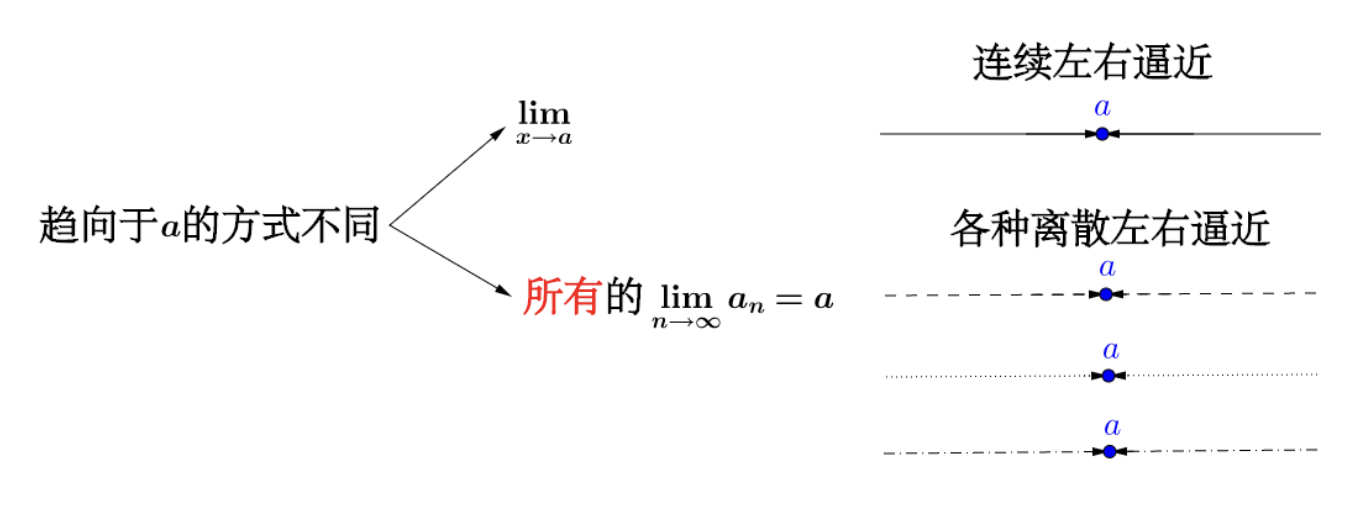
\includegraphics[width=
            0.9 \linewidth]{2.2.1.png}
    \end{figure}
    除此之外,$f(x)$ 和 $f(a_n)$的函数图像如下所示
    \begin{figure}[H] \centering
        \subfigure[函数$f(x)$图像] {
            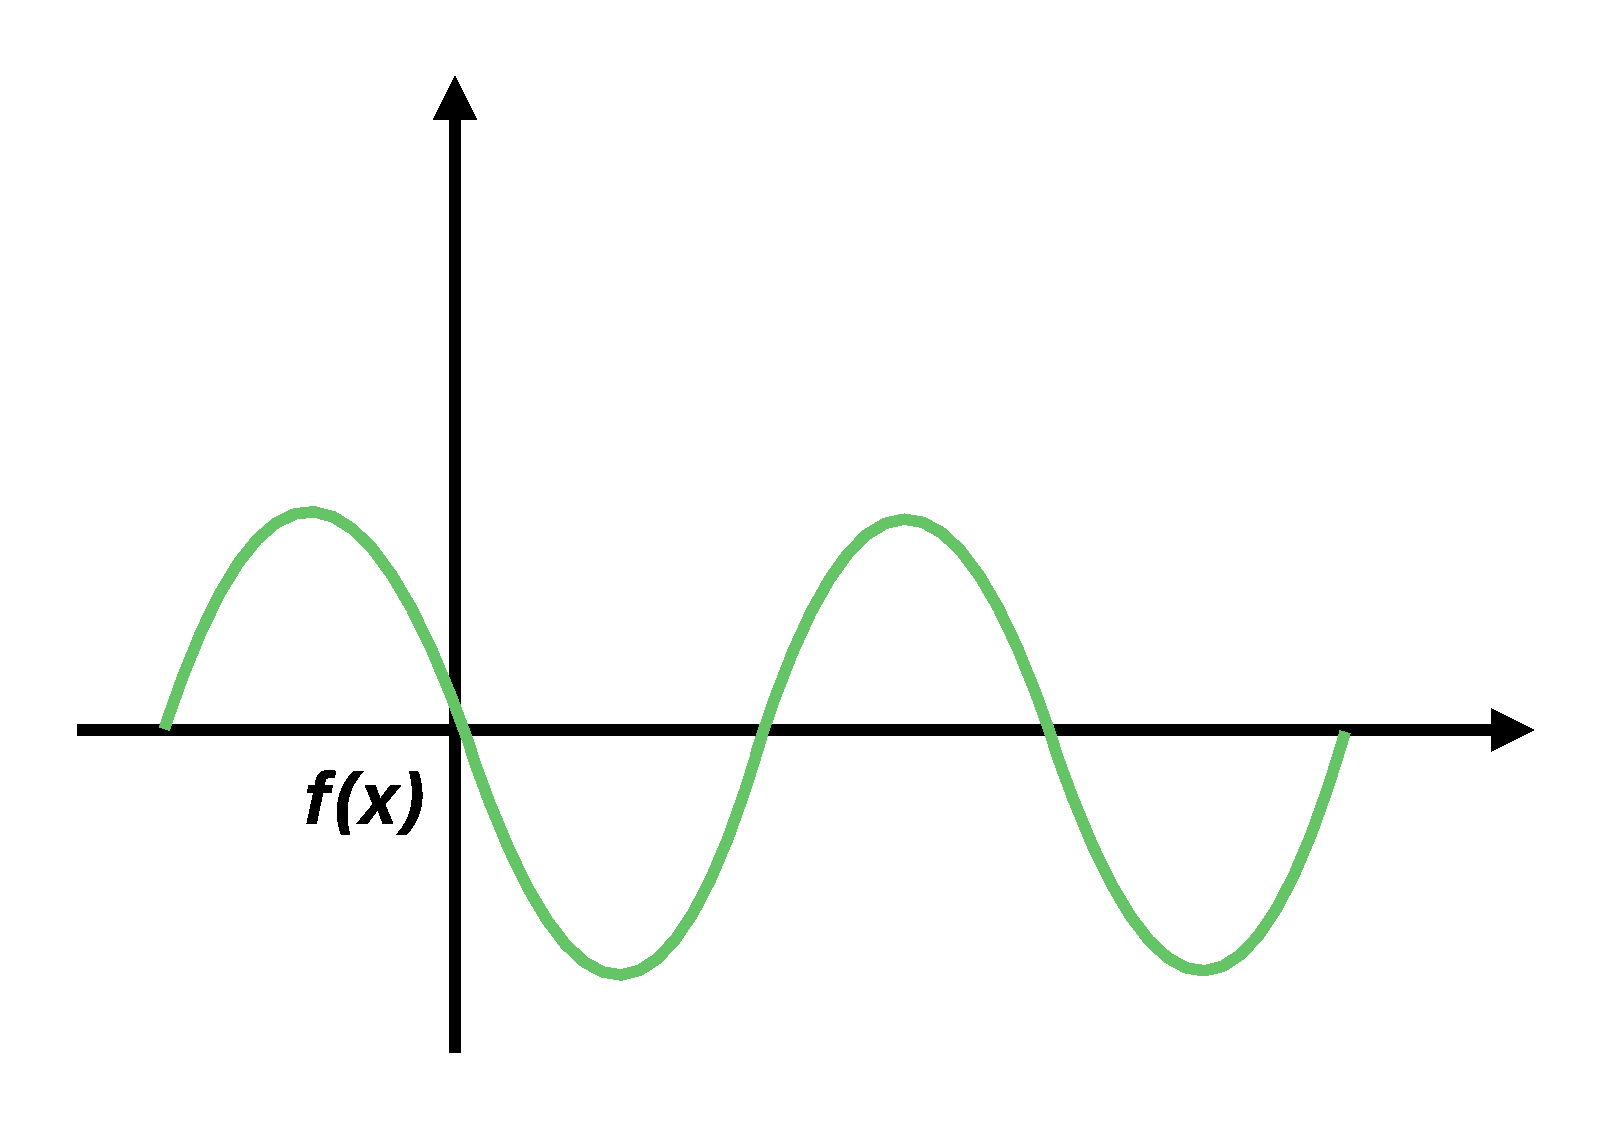
\includegraphics[width=0.45\columnwidth]{2.2.2.pdf}
        }
        \subfigure[函数$f(a_n)$图像] {
            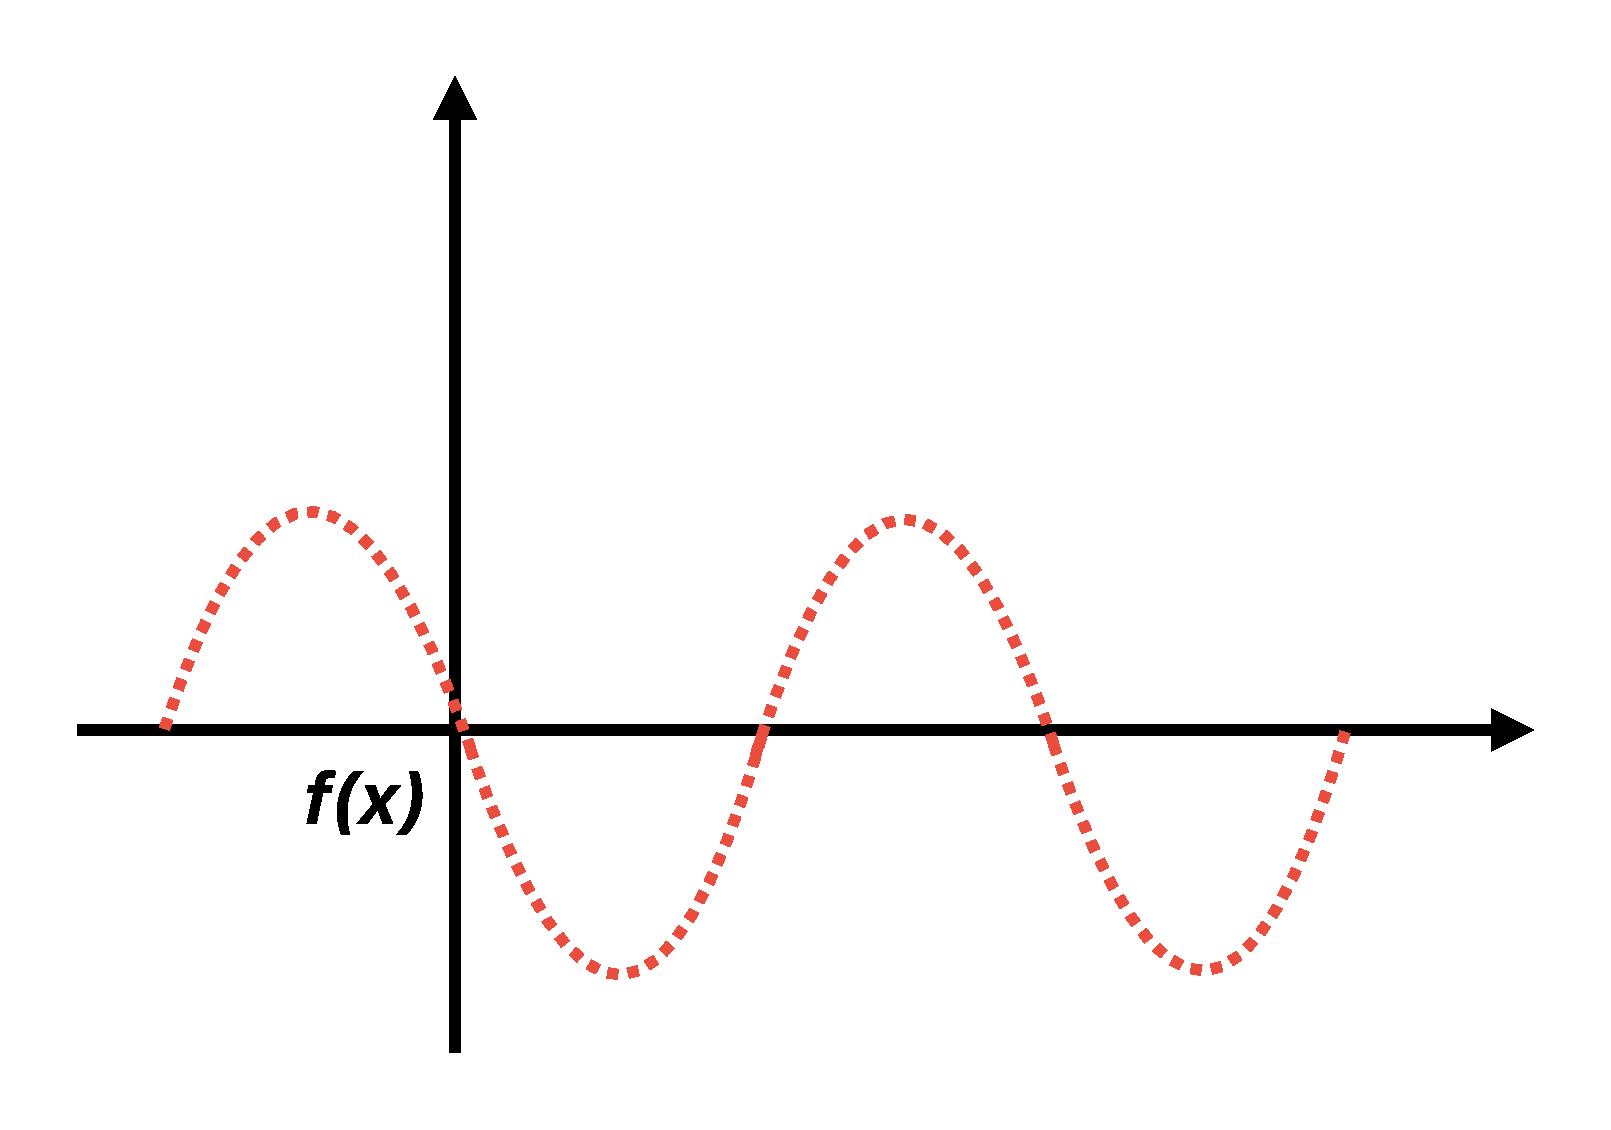
\includegraphics[width=0.45\columnwidth]{2.2.3.pdf}
        }
        \caption{$f(x)$与$f(a_n)$函数图像}
    \end{figure}

    \textcolor{red}{$f(a_n)$其实是$f(x)$的抽样}
    \begin{figure}[H]
        \centering 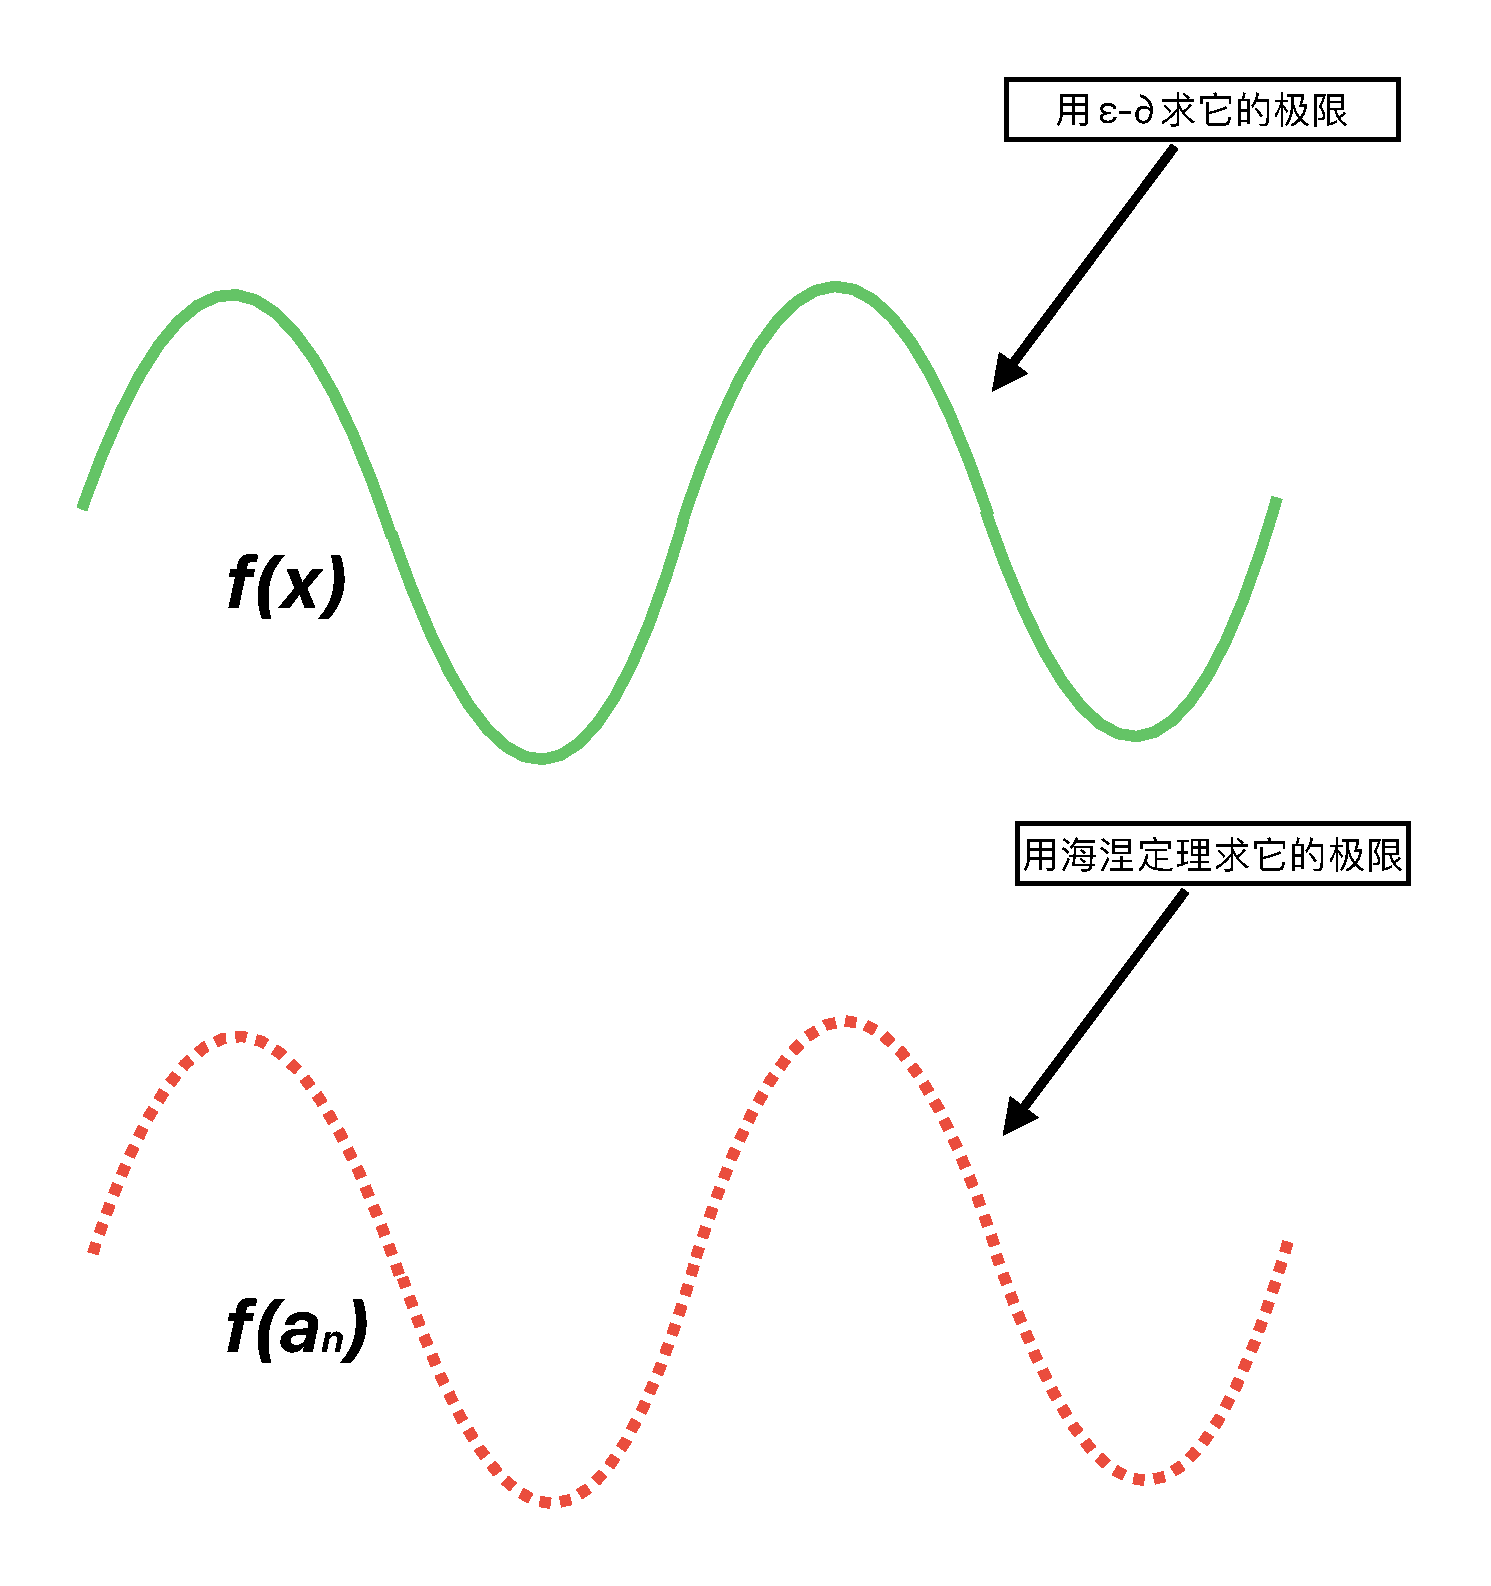
\includegraphics[width=
            0.4 \linewidth]{2.2.4.pdf}
    \end{figure}
    需要注意的是,是所有的数列(抽样)才能完全代表整体.不能说我选了某个数列有极限就代表函数有极限.

    总结:\textcolor{red}{海涅定理表述了离散与连续、数列极限与函数极限的关系.}
    \section{无穷小与无穷大}
    \subsection{无穷小}
    \begin{defn}{无穷小的定义}{}
        如果函数$f(x)$当$x\to x_0$(或 $x\to\infty$)时的极限为零,那么称函数$f(x)$为当$x\to x_0$(或$x\to\infty$)时的无穷小.
    \end{defn}
    \textbf{$f(x)$是可以本身为$0$或者无限趋近于零,其中$0$可以作为无穷小唯一常数}.
    \begin{criterion}{无穷小与函数极限的关系(脱帽法)}{}
        $\lim_{x\to\bullet}f(x)=A\Leftrightarrow f(x)=A+\alpha$,其中$\lim_{x\to\bullet}f(x)$为超实数值,其实数部分为$A$,函数$f(x)$的函数值为$A+\alpha$
    \end{criterion}
    \subsection{\textcolor{red}{无穷小的性质}}
    \begin{itemize}
        \item[1] 有限个无穷小的和是无穷小\footnote{无穷个无穷小的和不一定是无穷小,如$\lim_{n \to \infty}=(\frac{1}{n+1}+\frac{1}{n+2}+\frac{1}{n+3}\dots +\frac{1}{n+n})=\ln 2$}
            \begin{proof}
                设$\alpha_1$和$\alpha_2$为无穷小量。则$0 \leqslant |\alpha_1+\alpha_2|\leqslant |\alpha_1|+|\alpha_2|$,$|\alpha_1|+|\alpha_2|$的极限为0。证明完毕。
            \end{proof}
        \item[2] 有界函数与无穷小的乘积是无穷小\footnote{无界函数$\times$无穷小量不一定是无穷小,如$\lim_{x \to \infty}x \times \frac{1}{x}=1$}
            \begin{proof}
                $|\alpha _1|\leqslant M$,$\alpha_2$是无穷小量。那么$0\leqslant|\alpha_1 \times \alpha_2|=|\alpha_1|\times |\alpha_2|\leqslant M \times |\alpha_2|$证明完毕。
            \end{proof}
        \item[3] 有限个无穷小的乘积是无穷小\footnote{这个地方虽然张宇老师给出了证明,但是好像存在一定的争议性}
    \end{itemize}
    \subsection{\textcolor{red}{无穷小的比阶}}
    \begin{defn}{}{}
        \begin{itemize}
            \item 如果 $\lim \frac{\beta}{\alpha} =0$,那么就说 $\beta$是比$\alpha$高阶的无穷小,记作 $\beta=o(\alpha);$
            \item  如果 $\lim \frac\beta\alpha  =\infty$,那么就说 $\beta$是比 $\alpha$低阶的无穷小;
            \item 如果$\lim\frac{\beta}{\alpha} =c\neq 0$,那么就说 $\beta$ 与 $\alpha$ 是同阶无穷小 ;
            \item 如果$\lim\frac{\beta}{\alpha^{^k}} =c \neq 0$,$k > 0$,那么就说 $\beta$是关于 $\alpha$的$k$阶无穷小\footnote{不是相等,超实数系下没有加减运算,只可以进行替换运算};
            \item 如果 $\lim \frac\beta\alpha = 1$,那么就说 $\beta$ 与 $\alpha$ 是等价无穷小,记作 $\alpha\sim\beta$
        \end{itemize}
    \end{defn}
    前三个定义解释:$\lim \frac{\beta}{\alpha} =0$是指分子趋于$0$的速度比分母快,$\lim \frac\beta\alpha  =\infty$是指分子趋于$0$的速度比分母慢,$\lim\frac{\beta}{\alpha} =c\neq 0$是指趋于$0$的速度一样.

    同时需要注意的是,\textbf{并不是任意两个无穷小都可进行比阶的}.例如,当 $x\to 0$ 时,$x\sin\frac1x$与$x^2$虽然都是无穷小,但是却不可以比阶,也就是说既无高低阶之分,也无同阶可言,因为$\lim_{x \to 0}\frac{x \sin \frac{1}{x}}{x^2}=\lim_{x\to0}\frac1x\sin\frac1x$不存在,其值为$\infty$和$0$。
    \subsection{无穷小的运算}\footnote{此处多用于泰勒公式的应用中,会对上述高阶无穷小的运算提出要求}
    设$m,n$为无穷小,则
    \begin{itemize}
        \item[1.] $o(x^{m})\pm o(x^{n})=o(x^{l}),l=\min\{m,n\}$
        \item[2.] $o(x^{m})\bullet o(x^{n})=o(x^{m+n}),x^{m}\bullet o(x^{n})=o(x^{m+n})$
        \item[3.] $o(x^{m})=o(kx^{m})=k\bullet o(x^{m}),k \neq 0$
    \end{itemize}
    \subsection{无穷大}
    \begin{defn}{无穷大的定义}{}
        设函数$f(x)$在$x_0$的某一去心邻域内有定义(或$|x|$大于来一正数时有定义).如果对于任意给定的正数$M$(不论它多么大),总存在正数$\delta$(或数$X$),只要$x$适合不等式$0<|x-x_0|<\delta$(或$|x|>X$),对应的函数值$f(x)$总满足不等式
        $$
            |f(x)|>M
        $$
        那么称函数$f(x)$是当$x\to x_0$(或$x\to\infty$\footnote{等价于$x \to -\infty$同时$x \to +\infty$})时的无穷大.\footnote{\textbf{无穷大一定无界,但无界不一定是无穷大量。}与无穷小相同,都是一个极限过程,因此无穷大也是一个极限,所以无界不一定是无穷大量}
        其$\varepsilon-N$语言为
        $$
            \lim\limits_{x\to x_0}f(x)= \infty \Leftrightarrow\forall M >0,\exists\delta>0,\text{当}0<|x-x_0|<\delta\text{时},\text{有}|f(x)|>M.
        $$
    \end{defn}
    \begin{problem}
    证明$\underset{x\rightarrow1}{\operatorname*{lim}}\frac{1}{x-1}=\infty $
    \end{problem}
    \begin{solution}
        $\forall M>0$令$\delta=\frac{1}{4M}>0$,当$0<|x-1|<\delta$时,即$0<|x-1|<\frac{1}{4M}$时,$|x-1|<\frac{1}{M}$,所以$\frac{1}{|x-1|}>M$
        这就证明了$\underset{x\rightarrow1}{\operatorname*{lim}}\frac{1}{x-1}=\infty$
    \end{solution}
    \begin{criterion}{无穷大与无穷小的关系}{}
        在自变量的同一变化过程中,如果$f(x)$为无穷大,那么$\frac{1}{f(x)}$为无穷小;反之,如果$f(x)$为无穷小,且$f(x) \neq 0$,那么存在常数$\frac{1}{f(x)}为无穷大$
    \end{criterion}
    \subsection{\textcolor{red}{无穷大的比阶}}
    \begin{itemize}
        \item 当$x \to +\infty$时,$\mathrm{ln}^ax\ll x^\beta\ll a^x,\text{其中}\alpha>0,\beta>0,a>1.$\footnote{由洛必达公式证明}
        \item 当$n \to \infty$时,$\ln^an\ll n^\beta\ll a^n\ll n!\ll n^n,\text{其中 }\alpha>0,\beta>0,a>1.$
    \end{itemize}
    \subsection{\textcolor{red}{无穷大的性质}}
    \begin{itemize}
        \item 两个无穷大量的积仍未无穷大量
        \item 无穷大量与有界变量的和仍是无穷大量
    \end{itemize}
    \section{函数极限的运算}
    \subsection{极限的四则运算法则}
    如果极限不存在,那么极限属于超实数系的范畴,在超实数系下不可以进行代数运算,只可以进行替换运算。但是如果极限均存在,那么可以进行代数计算。\\
    若$\lim f(x)=A$,$\lim g(x)=B$,那么
    \begin{itemize}
        \item $\operatorname*{lim}[kf(x)\pm lg(x)]=k\operatorname*{lim}f(x)\pm l\operatorname*{lim}g(x)=kA\pm lB$,其中$k,l$为常数
        \item $\operatorname*{lim}[f(x)\bullet g(x)]=\operatorname*{lim}f(x)\bullet\operatorname*{lim}g(x)\equiv A\bullet B$,特别的,若$\lim f(x)$存在,$n$为正整数,则$\operatorname{lim}[f(x)]^n=\begin{bmatrix}\operatorname{lim}f(x)\end{bmatrix}^n$
        \item $\operatorname*{lim}\frac{f(x)}{g(x)}=\frac{\operatorname*{lim}f(x)}{\operatorname*{lim}g(x)}=\frac{A}{B}(B\neq0)$
    \end{itemize}
    \begin{criterion}{常用结论}{}
        \begin{itemize}
            \item 存在 \pm 不存在 = 不存在(只有这一个是不存在,其余都是不一定或者存在)
            \item 不存在 \pm 不存在 =不一定\footnote{反例:$\lim _{x \to 0}(\sin \frac{1}{x}-\sin \frac{1}{x})=0$}
            \item 存在 \times (\div) 不存在 = 不一定
            \item 不存在 \times (\div) 不存在 = 不一定
            \item 若$\lim f(x) = A \neq 0$,则$\lim f(x)\lim g(x)=A \times \lim g(x)$
        \end{itemize}
    \end{criterion}
    \begin{problem}
    \textbf{若$\lim \frac{f(x)}{g(x)}=A \neq 0$,则$\lim f(x)=0 ,\lim g(x)=0 $}
    \end{problem}
    \begin{proof}
        $g(x)=\frac{f(x)}{\frac{f(x)}{g(x)}}$。求极限得$\lim g(x)=\lim \frac{f(x)}{\frac{f(x)}{g(x)}}=\frac{\lim f(x)}{\lim \frac{f(x)}{g(x)}}=0$.证明完毕\footnote{此证明为结论,经常使用}。
    \end{proof}
    \subsection{洛必达法则}
    \begin{defn}{}{}
        \begin{itemize}
            \item $\lim_{x\to x_0}f(x)=\lim_{x\to x_0}g(x)=0(\infty)$
            \item $f(x)$和$g(x)$在$x_0$的某去心邻域内可导,且$g'(x) \neq 0$
            \item $\lim_{x\to x_0}\frac{f^{\prime}(x)}{g^{\prime}(x)}\text{ 存在(或 }\infty)$
        \end{itemize}
        则$\lim_{x\to x_{0}}\frac{f(x)}{g(x)}=\lim_{x\to x_{0}}\frac{f^{'}(x)}{g^{'}(x)}$
    \end{defn}
    \textbf{需要注意的是使用过洛必达法则之后的极限必须存在,即$\lim _{x \to x_0}\frac{f'(x)}{g'(x)}$ 必须存在.}
    \begin{problem}
    求$\lim _{x \to 0}\frac{x^2 \times \sin \frac{1}{x}}{\sin x}$
    \end{problem}
    \begin{solution}
        该函数也是$\frac{0}{0}$型,但是如果使用洛必达法则,则$2x \times \sin \frac{1}{x}-\cos \frac{1}{x}$,极限显然不存在,因此不可以使用洛必达法则。则正确求法为$\lim _{x\to 0}\frac{x^2\times \sin \frac{1}{x}}{x}=\lim_{x\to 0}x\times\sin\frac{1}{x}=0$.
    \end{solution}
    \subsection{泰勒公式}
    设$f(x)$在点$x=0$处$n$阶可导\footnote{泰勒公式是在一点处展开,函数必须在那一点处n阶导数存在},则存在$x=0$的一个邻域,对于该领域内的任一点$x$,有:
    $$
        f(x)=f(0)+f'(0)x+\frac{f''(0)}{2!}x^2+\cdots+\frac{f^{(n)}(0)}{n!}x^n+o(x^n)
    $$
    当$x\to 0$时,有以下结论
    \begin{align*}
        \boxed{\begin{aligned}
                        & \sin x =x-\frac{x^3}{3!}+o(x^3)                                &  & \cos x =1-\frac{x^2}{2!}+\frac{x^4}{4!}+o(x^4)                  \\
                        & \arcsin x =x+\frac{x^3}{3!}+o(x^3)                             &  & \tan x =x+\frac{x^3}3+o(x^3)                                    \\
                        & \arctan x =x-\frac{x^{3}}{3}+o(x^{3})                          &  & \ln(1+x) =x-\frac{x^{2}}{2}+\frac{x^{3}}{3}+o(x^{3})            \\
                        & \mathrm{e}^{x} =1+x+\frac{x^{2}}{2!}+\frac{x^{3}}{3!}+o(x^{3}) &  & (1+x)^{a} =1+\alpha x+\frac{\alpha(\alpha-1)}{2!}x^{2}+o(x^{2}) \\
                   \end{aligned}}
    \end{align*}
    \begin{criterion}{泰勒公式应用时的展开原则}{}
        \begin{itemize}
            \item $\frac{A}{B}$型,适用于"上下同阶"原则:具体来说,如果分母或者分子是$x$的$k$次幂,则应把分子或分母展开到$x$的$k$次幂。如:$\lim_{x\to0}\frac{x-\ln(1+x)}{x^{2}}$,此处$\ln(1+x)$应展开为$x-\frac{x^2}{2}+o(x^2)$
            \item $A-B$型,适用"幂次最低"原则:将$A,B$分别展开到他们系数不相等的$x$的最低次幂为止。如:已知当$x\to0$时,$\cos x-e^{\frac{x^2}2}$与$ax^b$为等价无穷小,求$a,b$.则应展开为$\cos x=1-\frac{x^2}{2!}+\frac{x^4}{4!}+o(x^4),\mathrm{e}^{-\frac{x^2}{2}}=1-\frac{x^2}{2}+\frac{1}{2!}\frac{x^4}{4}+o(x^4).$
        \end{itemize}
    \end{criterion}
    \subsection{极限存在准则的两个应用(两个重要极限)}
    $$
        \lim _ { \square \rightarrow \infty } ( 1 + \frac { 1 } { \square } ) ^ { \square } = e
    $$
    \\
    $$
        \lim _ { \square \rightarrow 0 } \frac { \sin \square } { \square } = 1
    $$

    \subsection{夹逼准则}
    \begin{defn}{函数极限存在准则}{}
        如果
        \begin{itemize}
            \item 当$x\in U^{\circ}(x_{0},r)($ 或 $|x|>M)$ 时
                  $$
                      g(x)\leqslant f(x) \leqslant h(x)
                  $$
            \item $\lim_{x\to x_0(x\to\infty)}g(x)=A,\lim_{x\to x_0(x\to\infty)}h(x)=A$
        \end{itemize}
        那么$\lim_{x\to x_0(x\to\infty)}f(x)$存在,且等于$A$.
    \end{defn}
    \begin{itemize}
        \item 夹逼准则处主要通过放缩来求极限
        \item 常用的结论有:若$\lim _{n \to \infty} \sqrt[n]{a_1^n+a_2^n+...+a_m^n}$,其中$a_i >0(i=1,2,3,...,m)$,令$\max{a_i}=a$,则$\sqrt[n]{a^n}\leqslant\sqrt[n]{a_1^n+a_2^n+\cdots+a_m^n}\leqslant\sqrt[n]{ma^n}$,\\$\lim_{n\to\infty}\sqrt[n]{a^n}=a,\lim_{n\to\infty}\sqrt[n]{m\cdot a^n}=a$,则$\operatorname*{lim}_{n\to\infty}\sqrt[n]{a_1^n+a_2^n+\cdots+a_m^n}=a$
    \end{itemize}
    \subsection{\textcolor{red}{单调有界准则}}
    \begin{defn}{函数的单调有界准则}{}
        设函数$f(x)$在点$x_0$的某个左邻域内单调并且有界,则$f(x)$在$x_0$的左极限$f(x_0^-)$一定存在
    \end{defn}

    \subsection{函数极限的运算法则}
    \begin{defn}{}{}
        如果$\varphi(x)\geqslant\psi(x)$,而 $\lim\varphi(x)=A$, $lim \psi(x)=B$ ,那么 $A\geqslant B$
    \end{defn}
    \begin{defn}{复合函数极限运算法则}{}
        设函数$y=f[g(x)]$是由函数$u=g(x)$与函数$y=f(u)$复合而成,$f[g(x)]$在点$x_0$的某去心领域内有定义,若$\lim_{x \to  x_0} g(x)=u_0$,$\lim_{u \to u_0}f(u)=A$,且存在$\delta_0 >0$,当$x\in\mathring{U}\left(x_{0},\delta_{0}\right)$时,有$g\left(x\right)\neq u_{0}$,则
        $$
            \underset{x\to x_0}{\operatorname*{lim}}f[g(x)]=\underset{u\to u_0}{\operatorname*{lim}}f(u)=A.
        $$
    \end{defn}
    \begin{criterion}{常用的结论}{}
        \begin{itemize}
            \item $\lim f(x)=A \neq 0 \Rightarrow \lim f(x)g(x)=A \lim g(x)$
            \item $\lim \frac{f(x)}{g(x)}$存在,$\lim g(x)=0 \Rightarrow \lim f(x)=0$
        \end{itemize}
    \end{criterion}
    \subsection{等价无穷小替代}
    关于等价无穷小,有以下两个定理
    \begin{defn}{}{}
        $\beta$与$\alpha$是等价无穷小的充分必要条件为
        $$
            \beta=\alpha + o(\alpha)
        $$
    \end{defn}

    \begin{defn}{}{}
        设$\alpha\sim\widetilde{\alpha}$,$\beta\sim\widetilde{\beta}$,且$\lim\frac{\widetilde{\beta}}{\underset{\alpha}{\operatorname*{\sim}}}$存在,则
        $$
            \lim\frac{\beta}{\alpha}=\lim\frac{\widetilde{\beta}}{\overset{\sim}{\alpha}}.Í
        $$
        求两个无穷小之比的极限时,分子及分母都可用等价无穷小来代替.但是需要遵循以下代换原则\footnote{其实没有什么替换原则,本质其实是因为超实数系下不能进行实数运算,只能进行替换运算}
        \begin{itemize}
            \item 乘除关系可以换:若$\alpha\sim\alpha_1,\beta\sim\beta_1,\text{则}\lim\frac\alpha\beta=\lim\frac{\alpha_1}\beta=\lim\frac\alpha{\beta_1}=\lim\frac{\alpha_1}{\beta_1}$
            \item 加减关系一定条件下可以换
                  \begin{itemize}
                      \item 若$\alpha\sim\alpha_{1},\beta\sim\beta_{1},\text{且}\operatorname*{lim}\frac{\alpha_{1}}{\beta_{1}}=A\neq1,\text{则 }\alpha-\beta\sim\alpha_{1}-\beta_{1}$
                      \item 若$\alpha\sim\alpha_{1},\beta\sim\beta_{1},\text{且}\operatorname*{lim}\frac{\alpha_{1}}{\beta_{1}}=A\neq-1,\text{则 }\alpha+\beta\sim\alpha_{1}+\beta_{1}$
                  \end{itemize}
        \end{itemize}
        加减关系代换准则证明如下:
        \begin{proof}
            $$\lim \frac{\alpha-\beta}{\alpha_1 -\beta_1}=\lim \frac{\beta (\frac{\alpha}{\beta}-1)}{\beta_1(\frac{\alpha_1}{\beta_1}-1)}=1$$
        \end{proof}
    \end{defn}
    以下为常用等价无穷小
    \\当$x \to 0$时,有
    \begin{align*} \boxed{
            \begin{aligned}
                 & x \sim \sin x \sim \tan x \sim \arcsin x \sim \arctan x \nonumber \\
                 & \quad  \sim \ln (1+x)  \nonumber                                  \\
                 & \quad \sim e^x -1 \nonumber
            \end{aligned} }
    \end{align*}

    \begin{align*} \boxed
        {
            \begin{aligned}
                 & (1+x)^a \sim  1+ax   \\
                 & a^x - 1 \sim x \ln a
            \end{aligned}
        }
    \end{align*}
    \begin{criterion}{上述结论的推广}{}
        当$x \to 0$时,若$(1+x)^a -1 \sim ax$,则$\alpha (x) \to 0,\alpha(x)\beta(x) \to 0$,则
        $$
            [1+\alpha(x)]^{\beta(x)} -1 \sim \alpha(x) \beta(x)
        $$
    \end{criterion}
    \begin{align*} \boxed
        {
            \begin{aligned}
                 & \frac{1}{2} x^2 \sim 1-\cos x \sim \sec x -1 \sim x- \ln(1+x)
            \end{aligned}
        }
    \end{align*}

    \begin{align*} \boxed
        {
            \begin{aligned}
                 & \frac{1}{6} x^3 \sim x-\sin \sim \arcsin x -x
            \end{aligned}
        }
    \end{align*}
    \begin{align*} \boxed
        {
            \begin{aligned}
                 & \frac{1}{3} x^3 \sim x-\arctan x \sim \tan x-x
            \end{aligned}
        }
    \end{align*}
    \subsection{利用基本极限求极限}
    \begin{align*} \boxed
        {
            \begin{aligned}
                 & \lim_{\square \to \infty }(1+|\square|)^{\frac{1}{\square}}=e^{|\square| \frac{1}{\square}} \qquad     \lim _ { \square \rightarrow 0 } \frac { \sin \square } { \square } = 1 \\
                 & \lim_{n \to \infty }\sqrt[n]{n}=1 \qquad \lim_{n \to \infty} \sqrt[n]{a}=1(a>0)                                                                                                \\
                 & \lim_{x \to 0} \frac{a^x-1}{x}=\ln a
            \end{aligned}
        }
    \end{align*}
    \subsection{定积分求极限}
    \subsection{七种未定式的计算}
    \subsubsection{形如$\frac{0}{0}$,$\frac{\infty}{\infty}$,$0 \times \infty$}
    \subsubsection{形如$\infty -\infty$}
    \subsubsection{形如$\infty^0,0^0$}
    \subsubsection{形如$1^{\infty}$}
    \section{数列极限的运算}
    \subsection{数列极限的运算法则}
    设$\underset{n\to\infty}{\operatorname*{lim}}x_{n}=a,\underset{n\to\infty}{\operatorname*{lim}}y_{n}=b$,则
    \begin{itemize}
        \item $\operatorname*{lim}_{n\to\infty}(x_n\pm y_n)=a\pm b$
        \item $\lim_{n\to\infty}x_{n}y_{n}=ab$
        \item 若$b \neq 0,y_n \neq 0$,则$\lim_{n\to\infty}\frac{x_n}{y_n}=\frac{a}{b}$
    \end{itemize}
    上述运算规则可推广至有限个数列的情况
    \subsection{夹逼准则}
    \begin{them}{数列极限存在准则}{}
        如果数列$\{|x_n|\},\{y_n\}$及$\{z_n\}$满足下列条件:
        \begin{itemize}
            \item 从某项开始,即$\exists n_0 \in N_+(\text{即}n \to \infty),$当$n>n_0$时,有
                  $$
                      y_n \leqslant x_n \leqslant z_n
                  $$
            \item $\lim_{n\to\infty}y_{n}=a,\operatorname*{lim}_{n\to\infty}z_{n}=a$
        \end{itemize}
        那么数列$\{ x_n \}$的极限存在,且$\lim_{n\to\infty}x_{n}=a$
    \end{them}
    \subsection{\textcolor{red}{单调有界准则}}
    \begin{them}{数列的单调有界准则}{}
        单调有界数列必有极限,即若数列$\{x_n\}$单调增加(减少)且有上界(下界),则$\lim_{n \to \infty} x_n$存在
    \end{them}
    %  ############################ 正文部分
    \ifx\allfiles\undefined
\end{sloppypar}
\end{document}
\fi
